% !TEX root =./main.tex

\section{Conclusion}
We successfully implemented all stages of the sonar system except for image sharpening. The final image produced 
matches the reference image provided with the project materials. We rearranged the stages somewhat by moving bias 
removal into stage 3 (band limiting and denoising) and rearranging the stages so that stage 3 came first, followed 
by stage 1, stage 2, stage 4, and stage 5. The purpose of that was to allow for a simpler, more reliable method
of implementing the required functionality. Overall, we aimed for quality first, then speed, which is reflected
in our manner of implementation in code. We used vector operations where possible and minimized unnecessary
memory copies or needless recalculations.

In the second half of this exercise, we learned from the mistakes of the first half that led to version control 
chaos and sub-optimal performance in some stages. To maintain speed, we used vector operations instead of loops 
and pre-computed tables whereever feasible, and in the one case where loops were unavoidable, we used low-level 
optimized C instead of MATLAB. The end result is a sonar system which is high-quality yet relatively efficient.

The primary challenge we faced was, in fact, not even in the actual work in \textsc{MATLAB}. Instead, a bigger source
of issues was the Git version control system, which caused conflicts and even odd glitches in earlier drafts of this 
report. The lesson from that experience is that often times, it is not the actual engineering and building which causes 
issues, but all the things surrounding and supporting those. Active communication and coordination before and during 
version control operations helped alleviate many of these issues.

\begin{figure}[H]
    \centering
    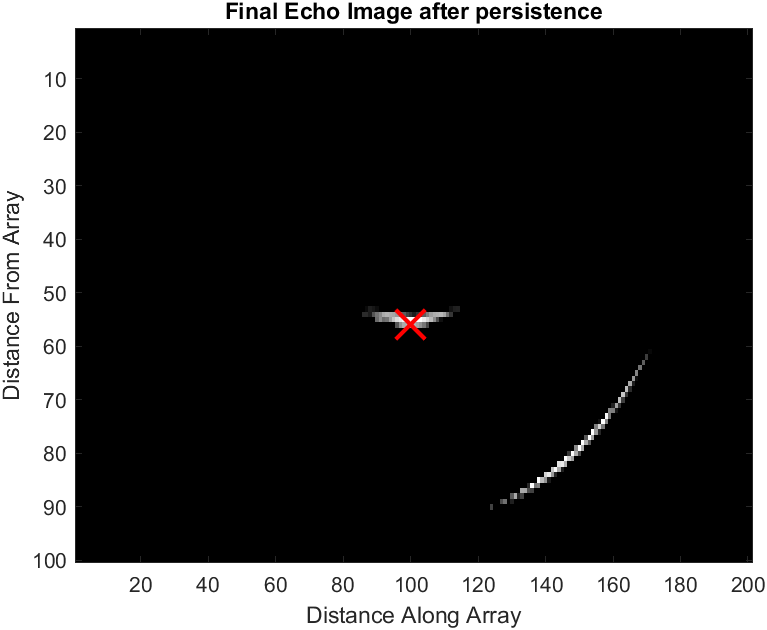
\includegraphics[width=0.5\linewidth]{figures/finalImage.png}
    \caption{Final Output Image}
    \label{fig:final_image}
\end{figure}

\section*{Documentation}
We worked as a team on this project. Additionally, we used resources such as the Mathworks website for \textsc{MATLAB} 
syntax help (ex, confirming how to index every other entry of a matrix). Example code included with the MATLAB 
installation was used as a starting point for the native C library. We also had a discussion with ChatGPT regarding 
recording phase, available \href{https://chatgpt.com/c/673ff615-bf94-800b-a437-6f861b769c24}{at this link}. 
We also used that same ChatGPT conversation to discuss the mathematics behind accounting for time gain compensation.